%
% Florent JACQUET - Antonin Waltz
%
% Rapport de LO43 (A14)
%   SmallUTBMworld
%
%
\documentclass[a4paper]{report}
%packages
\usepackage[utf8]{inputenc}
\usepackage[francais]{babel}
\usepackage{graphicx}\graphicspath{{pictures/}}
\usepackage{float}
\usepackage[T1]{fontenc}
\usepackage{color}
\usepackage{fancyhdr}
\usepackage{listings}
\usepackage[colorlinks=true,allcolors=black]{hyperref}
\usepackage[font=small,labelfont=bf,margin=\parindent,tableposition=top]{caption}
\setcounter{tocdepth}{2}
\begin{document}
\begin{titlepage}
    
\includegraphics[width=0.4\textwidth]{logo_utbm.png}
    \begin{center}
        \textsc{\LARGE Université de Technologie de Belfort Montbéliard}\\[1cm]
        \textsc{\Large LO43}\\
        \rule{\linewidth}{0.5mm}
        { \huge \bfseries Smallworld UTBM\\[0.4cm] }
        \rule{\linewidth}{0.5mm}
        \vskip1cm
        % Author and supervisor
        Florent \textsc{Jacquet}\\
        Antonin \textsc{Waltz}\\
        Superviseur: Amine \textsc{Ahmed Benyahia}\\
        \vskip1cm
        %\includegraphics[width=0.6\textwidth]{smallworld.png}
        \vfill
        {\large Automne 2014}
    \end{center}
\end{titlepage}
\newpage
\tableofcontents
\listoffigures
\newpage
\chapter{Présentation du projet}
\par
Durant ce semestre en LO43, nous avons choisi le projet \textit{Smallworld}
parmi tout ceux proposés.
\par
\textit{Smallworld} est un jeu de stratégie qui propose de gérer la destinée de
peuples fantastiques, chacun disposant d'une particularité unique. En plus de
ça, ceux-ci sont associés aléatoirement à un pouvoir spécial qui leur confére
une capacité supplémentaire.
\par
Le but est de conquérir des territoires afin d'obtenir le plus de points de
victoire. Cependant au fur et à mesure de l'avancé du jeu, un peuple a tendance
à s'affaiblir.  Le joueur qui le contrôle peut alors le faire passer en déclin
et choisir une nouvelle civilisation.
\par
Nous avons adapter les peuples et les pouvoirs à l'environnement de l'école, en
respectant les régles de base du jeu.
\newpage
\chapter{Organisation et répartition du travail}
\par
Notre groupe étant composé de 2 personnes, il était facile pour nous de
communiquer sur l'avancé du projet, la façon d'aborder telle où telle contrainte
technique où fonctionnelle ou tout simplement faire le point.
\par
Dans un premier temps et après nous être approprié \textit{Smallworld}, nous
avons réaliser les spécifications UML ensemble afin de partir sur la même base
de départ. Evidemment nous adapterons au fur et à mesure de l'implémentation en
fonction de l'évolution des contraintes. Nous nous sommes également mis d'accord
sur l'utilisation du pattern MVC, du polymorphisme, etc.
\par
Concernant les outils, nous avons utilisé \textbf{Eclipse}, \textbf{Dia} pour
l'UML et un dépôt \textbf{Git} pour la synchronisation des sources et le
versionnage. Nous avons également profiter des fonctionnalités de \textbf{Git}
pour effectuer un suivi efficace des fonctions à modifier où terminer.
\par
La répartition du travail s'est globalement fait ainsi, sachant que chacun
n'hésitait pas à intervenir dans les parties de l'autre si besoin était et qu'elle n'est pas définitive :
\begin{itemize}
    \item Florent : Modèle, Contrôleur, Rapport
    \item Antonin : Vue, Rapport
\end{itemize}
\newpage
\chapter{Architecture du projet}
\section{Première approche (Cas d'utilisation)}
Lorsque l'utilisateur lance le jeu, un premier menu s'offre à lui. Il peut choisir entre lancer une nouvelle partie, charger une partie déjà existante, afficher les règles où quitter le jeu.
\par Le seul cas qu'il est intéressant de détailler est celui d'une nouvelle partie. Après que le nombre de joueur ait été défini, les utilisateurs jouent chacun à tour de rôle. Ils ont alors le choix entre 4 actions :
\begin{itemize}
\item Acheter un peuple
\item Passer en déclin
\item Attaquer un terrain
\item Se redéployer
\end{itemize}
L'ordre et les différentes interactions entre ces actions sont détaillés dans le diagramme de séquence.
\section{Le modèle}
\par
C'est là le cœur du programme. Le modèle est une classe qui regroupe toutes les
classes du jeu en lui même, c'est à dire la carte, les jetons, les joueurs où
toute autre classe utile à la simulation du jeu par le programme.  En revanche, il ne s'agit
nullement de l'affichage, puisque cette tâche est laissée à la
partie Interface Utilisateur, la Vue.
\par
Cette partie est la seule pour laquelle nous avons réalisé un diagramme de
classe, étant donné qu'elle représente une grosse partie du projet, et que
beaucoup de classes entrent en jeu. Afin de mieux le structurer et de
savoir toujours dans quelle direction partir, le diagramme UML se trouvant en
Annexe 3 a été réalisé. Cela a permis d'avoiruimmédiatement un aperçu de
l'implémentation globale, et de se mettre d'accord sur la conception du projet.
\section{L'interface (la Vue)}
Lors d'un tour de jeu, le joueur doit pouvoir effectuer les actions qu'il désire. En même temps il est nécessaire qu'il ait accès à toutes les informations utiles.
\par
L'interface se divise en 4 parties distinctes :
\begin{itemize}
\item En haut, un récapitulatif des informations de base des joueurs adversaires : pseudo, peuple et pouvoir actif, icône d'avatar etc.
\item À droite, la liste des combinaisons peuple-pouvoir avec le nombre de pièces d'or correspondantes qu'il est possible de choisir.
\item Au centre, le plateau de jeu avec les territoires, le peuple par territoire, les attributs spéciaux etc.
\item En bas, les informations relatives au joueur actif, ainsi que les boutons d'action
\end{itemize}
Elle est cependant susceptible d'évoluer lors de l'implémentation.
\section{Le déroulement d'une phase de jeu (Séquence)}
\par
Cette partie est très importante, puisqu'il s'agit en somme des règles du jeu.
Étant donné que le programme est évènementiel, il suffit de savoir
quelle action peut être faite à quel moment, et cela se résume dans le
diagramme de séquence que nous avons fait, qui se trouve en Annexe 2.
\par
Ce diagramme s'étend sur la séquence de jeu d'un joueur, ce qui ne
représente pas la séquence complète du programme, mais simplement la partie
essentielle de celle-ci. On omet donc les étapes de fin de tour, ainsi que celles
de l'initialisation et de la fin du jeu, qui ne sont pas \"essentielles\" au déroulement
d'une partie.
\newpage
\chapter{Réalisation}
\section{Menu d'accueil}
\par
Au lancement du jeu, l'utilisateur arrive sur la page du menu d'accueil. IL peut alors ajouter où retirer des joueurs, lancer une nouvelle partie, parcourir les règles du jeu, charger une partie déjà existante où encore quitter. Un bouton retour est également disponible afin de pouvoir retourner facilement sur l'accueil suivant la page affichée.
\section{Durant une partie}
\par
Lorsque l'on est en jeu, toutes les actions prévues dans les règles sont réalisables. On peut sélectionner un peuple, conquérir des territoires occupés où non, passer au joueur suivant et enfin passer en déclin. On dispose également des informations courantes, comme le nombre de jetons possédés où le peuple actif. On peut également à tout moment sauvegarder sa partie, quitter le jeu et la recharger via le menu principale. Toute la fenêtre de jeu est également redimensionnable en permanence, les éléments affichés s'adaptant en conséquence.
\section{Ce qui manque}
\par
Tout le jeu est fonctionnel, cependant nous n'avons pas implémenter les jetons spéciaux et les régles des pouvoirs. Ces dernières existent mais ne changent rien au déroulement de la partie. Nous n'affichons également pas les images correspondant à chaque combinaison peuple-pouvoir disponible. De la même manière, nous n'affichons pas les jetons posés dessus par les joueurs ayant sélectionné une combinaison plus haut dans la pile. Il manque également la présence initiale de jetons peuple neutre afin d'empêcher les joueurs de conquérir un trop grand nombre de territoire durant les premiers tours.
\section{Ce qui est différent du modèle UML}
\par
Durant l'implémentation, nous avons préféré changer l'héritage de spécialisation des cases du plateau, des peuples et des pouvoirs afin d'éviter une trop grande quantité de fichier et rendre l'arborescence du projet plus lisible. Désormais ce sont simplement des attributs type dans la sous-classe correspondante.
\chapter{Bilan}
\section{Conclusion}
\par
Le fait d'avoir à réaliser un jeu rendait le projet ludique et donnait envie de s'investir. Il nous a permis d'appliquer les concepts vus en cours, mais aussi d'avoir à aller chercher plus loin, que ce soit dans la documentation ou les possibilités offertes par le langage Java. Nous avons également dû utiliser des outils de versionnage, la maitrîse de ces outils ne pourra qu'être un plus dans notre carrière professionnelle.
\section{Améliorations possibles}
\par
Nous aurions pu améliorer notre jeu de la façon suivante :
\begin{itemize}
\item Nous aurions pu ajouter une musique d'ambiance ainsi que des effets sonores lors d'un évènement.
\item Il manque la grande carte pour pouvoir contenir un nombre de joueurs plus important.
\item Il manque l'implémentation des règles des pouvoirs.
\item Il manque l'affichage des jetons sur la pile de combinaisons.
\item Il manque l'implémentation des jetons spéciaux.
\item Le jeu serait plus intéressant si nous avions ajouté davantage de peuples et de pouvoirs.
\item Une page supplémentaire dans le menu afin de pouvoir configurer des options (graphiques, sons, etc.)
\end{itemize}
\newpage
\chapter{Annexes}
\section{Diagramme des cas d'utilisation}
\begin{figure}[H]
    \begin{center}
        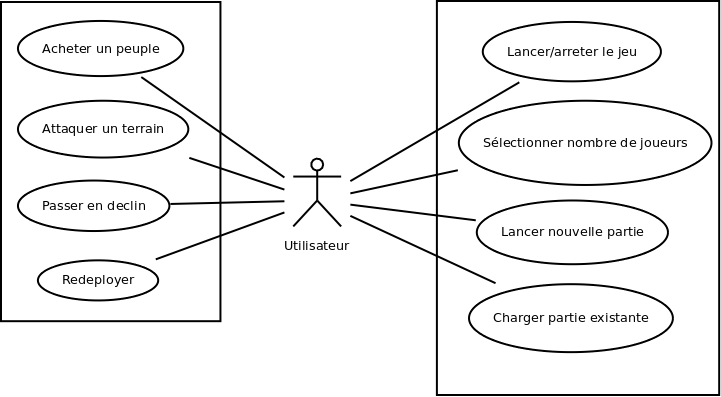
\includegraphics[width=0.85\textwidth]{use_case.png}
        \caption{Diagramme des cas d'utilisation du \textit{Smallworld}}
    \end{center}
\end{figure}
\section{Diagramme de séquence}
\begin{figure}[H]
    \begin{center}
        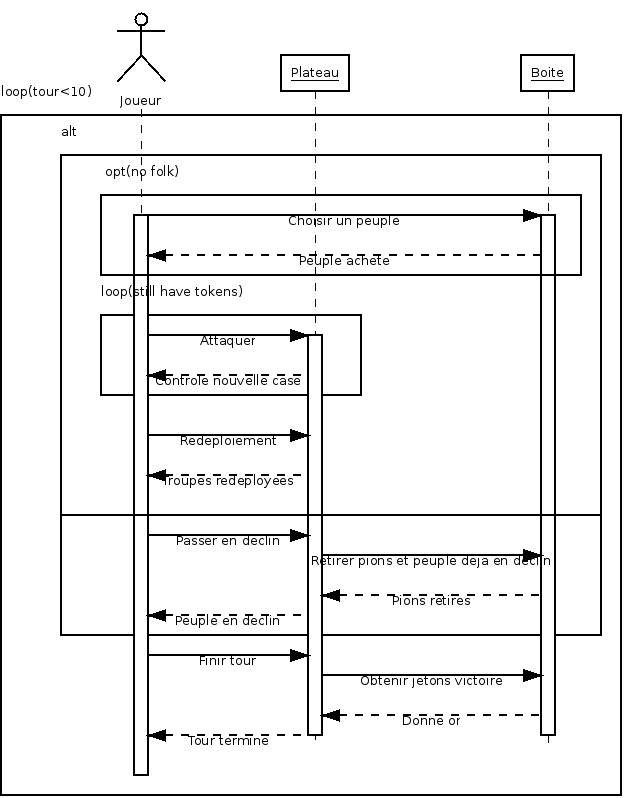
\includegraphics[width=0.85\textwidth]{sequence.png}
        \caption{Diagramme de séquence d'un tour de jeu}
    \end{center}
\end{figure}
\section{Diagramme de classes}
\begin{figure}[H]
    \begin{center}
        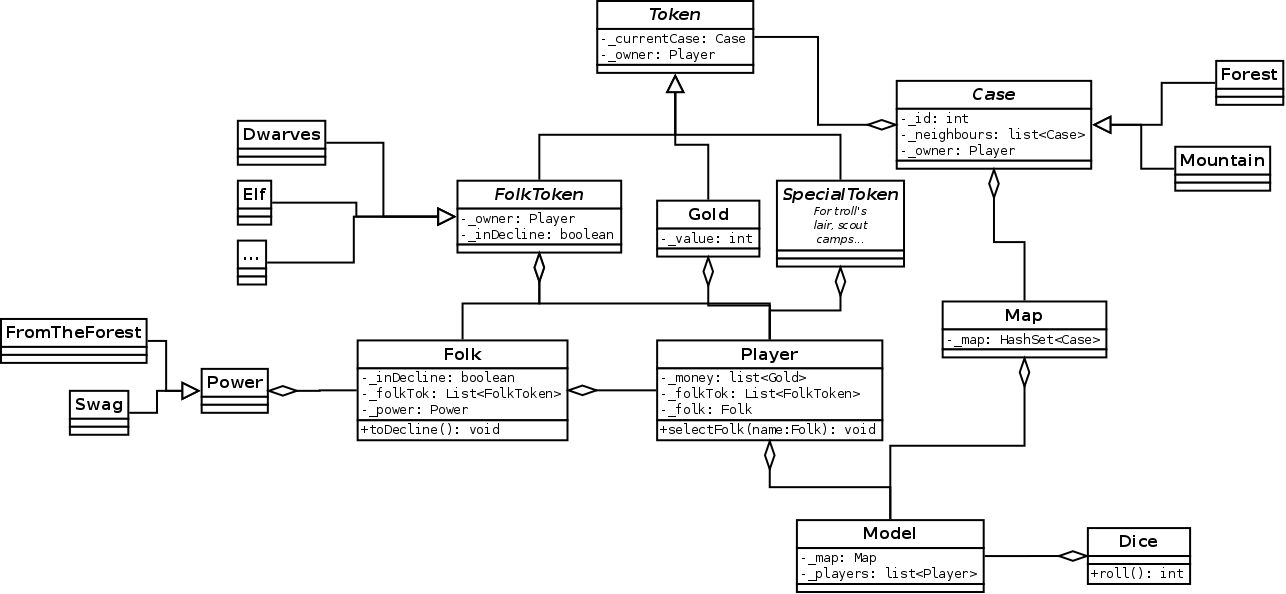
\includegraphics[width=0.85\textheight,angle=90]{classe.png}
        \caption{Diagramme de classe du modèle}
    \end{center}
\end{figure}
\section{Interface}
\begin{figure}[H]
    \begin{center}
        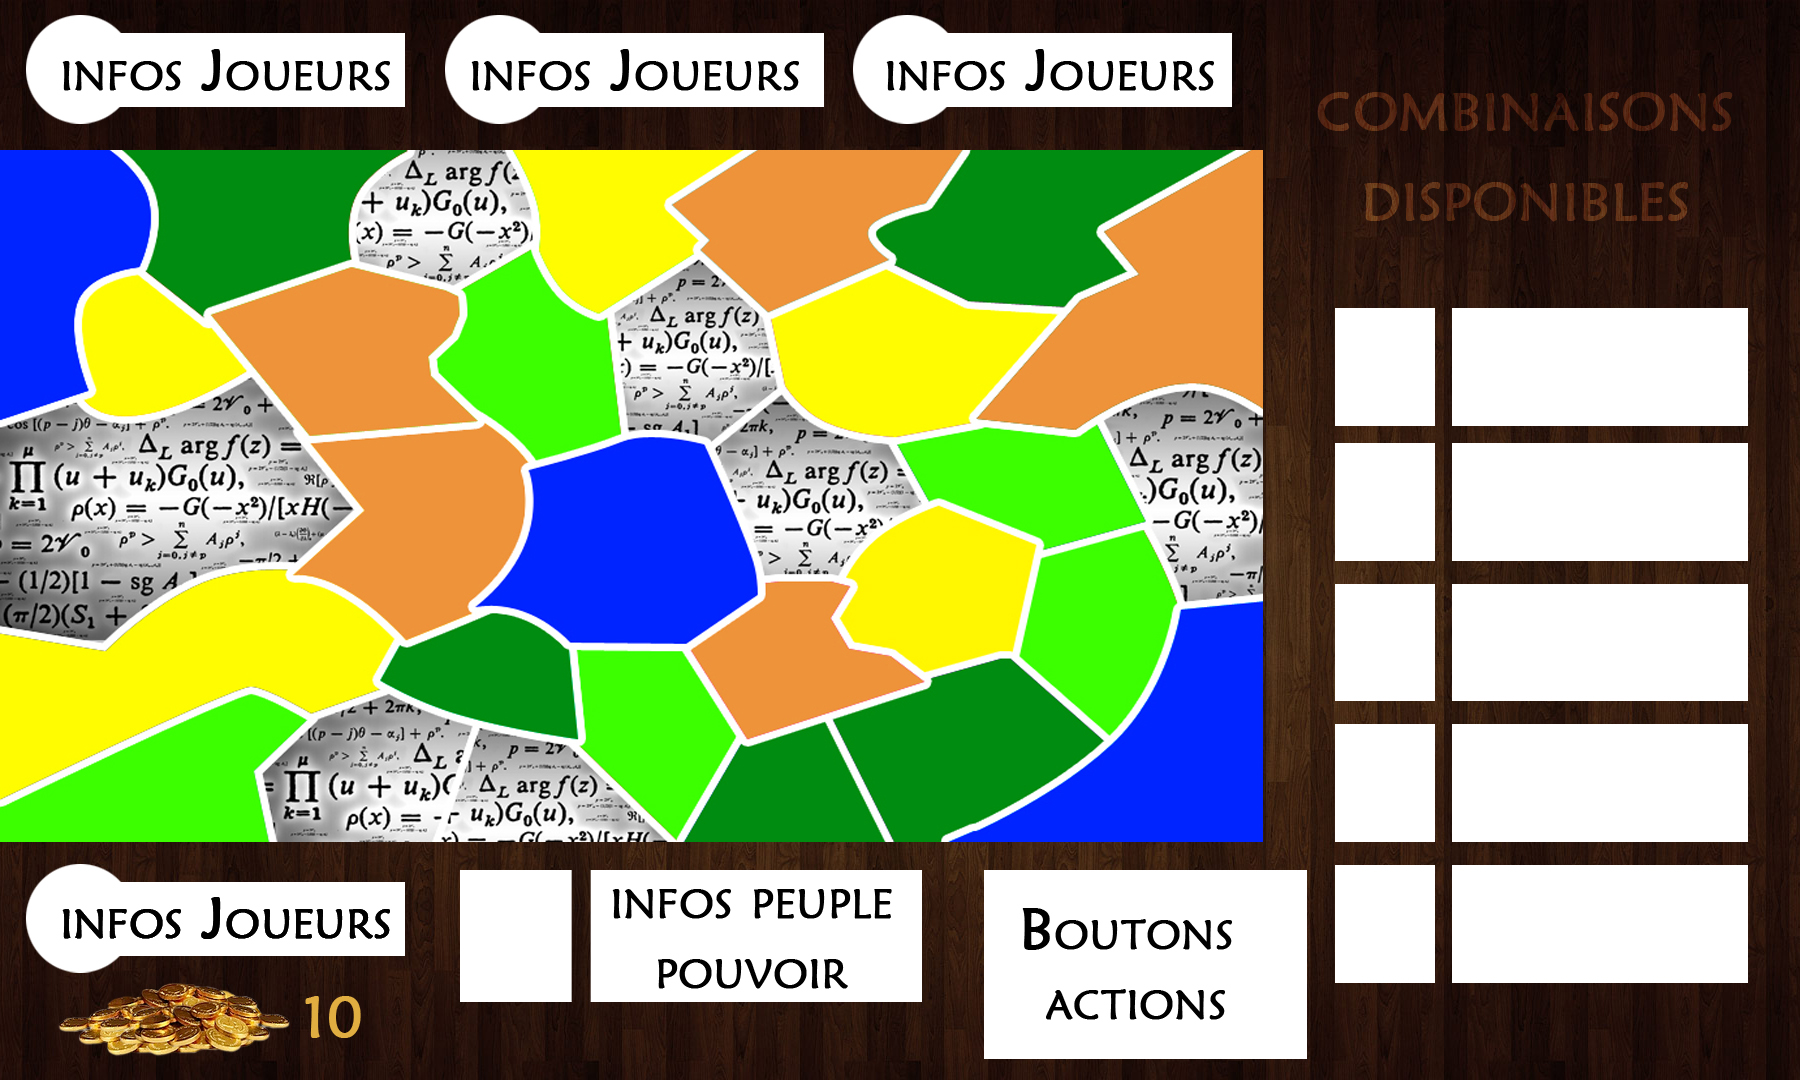
\includegraphics[width=0.85\textheight,angle=90]{plateau.jpg}
        \caption{Maquette de l'interface lors d'un tour de jeu}
   \end{center}
\end{figure}
\end{document}

